\footnotesize
\begin{tikzpicture}[>=latex]
\begin{axis}[
width=10cm,
height=7cm,
xtick=\empty,
ytick=\empty,
axis x line=center,
axis y line=center,
xlabel={$\lambda$},
ylabel={$f$},
xlabel style={right},
ylabel style={left},
xmin=0,xmax=4.5,ymin=0,ymax=1.7]
\addplot[dashed,line width=.4mm,color=black,mark=none,domain=0:.8]{1.5625};
\addplot[dashed,samples=40,line width=.4mm,color=black,mark=none,domain=.8:4]{1/x/x};
\addplot[name path=A,line width=1mm,color=black,mark=none,domain=0:.9]{1.234567901};
\addplot[name path=B,samples=40,line width=1mm,color=black,mark=none,domain=.9:4]{1/x/x};
\addplot[dashed,very thick,mark=none,domain=0:1.5]{1.234567901}node[right,pos=1,align=center]{reduced strength\\due to local buckling};
\addplot[name path=C,domain=0:.9]{0};
\addplot[name path=D,domain=.9:4]{0};
\addplot[00cc66,opacity=.3]fill between[of=A and C];
\addplot[00cc66,opacity=.3]fill between[of=B and D];
\node[align=center]at(.5,.6){safe\\region};
\end{axis}
\node[anchor=center]at(12,2.7){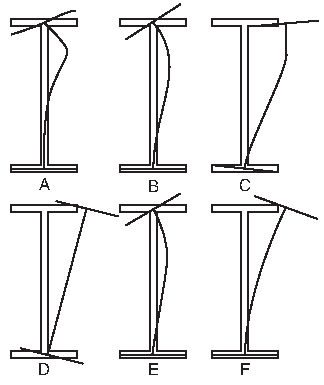
\includegraphics[height=6cm]{PIC/CH04/LB}};
\end{tikzpicture}